\documentclass[tikz,border=0pt]{standalone}
\usepackage[T1]{fontenc}
\usetikzlibrary{arrows.meta,backgrounds,shapes.geometric}
\usepackage[sfdefault,lining]{FiraSans}
\definecolor{ink}{HTML}{23373B}
\definecolor{accent}{HTML}{EB811B}
\definecolor{primary}{HTML}{9FCFCC}
\definecolor{store}{HTML}{D3DADD}
\definecolor{zone}{HTML}{F2F5F6}
\tikzset{
 box/.style={draw=none,rounded corners=2pt,fill=white,minimum height=13mm,text width=29mm,align=center,inner sep=3pt},
 component/.style={box,fill=primary},
 actor/.style={box,draw=ink,line width=.6pt,rounded corners=6.5mm,text width=28mm},
 external/.style={box,draw=ink,line width=.6pt,dashed,text width=34mm},
 flow/.style={-{Stealth[length=2.2mm]},draw=accent,line width=.9pt},
 status/.style={-{Stealth[length=2.2mm]},draw=ink,dashed,line width=.7pt},
 data/.style={{Stealth[length=1.8mm]}-{Stealth[length=1.8mm]},draw=ink!70,densely dotted,line width=.8pt},
 el/.style={font=\sffamily\fontsize{9}{11}\selectfont,fill=zone,inner sep=2pt,align=center},
 heading/.style={font=\sffamily\bfseries\fontsize{11}{13}\selectfont,text=ink},
 note/.style={font=\sffamily\fontsize{9}{12}\selectfont,align=left,text=ink}
}
\begin{document}
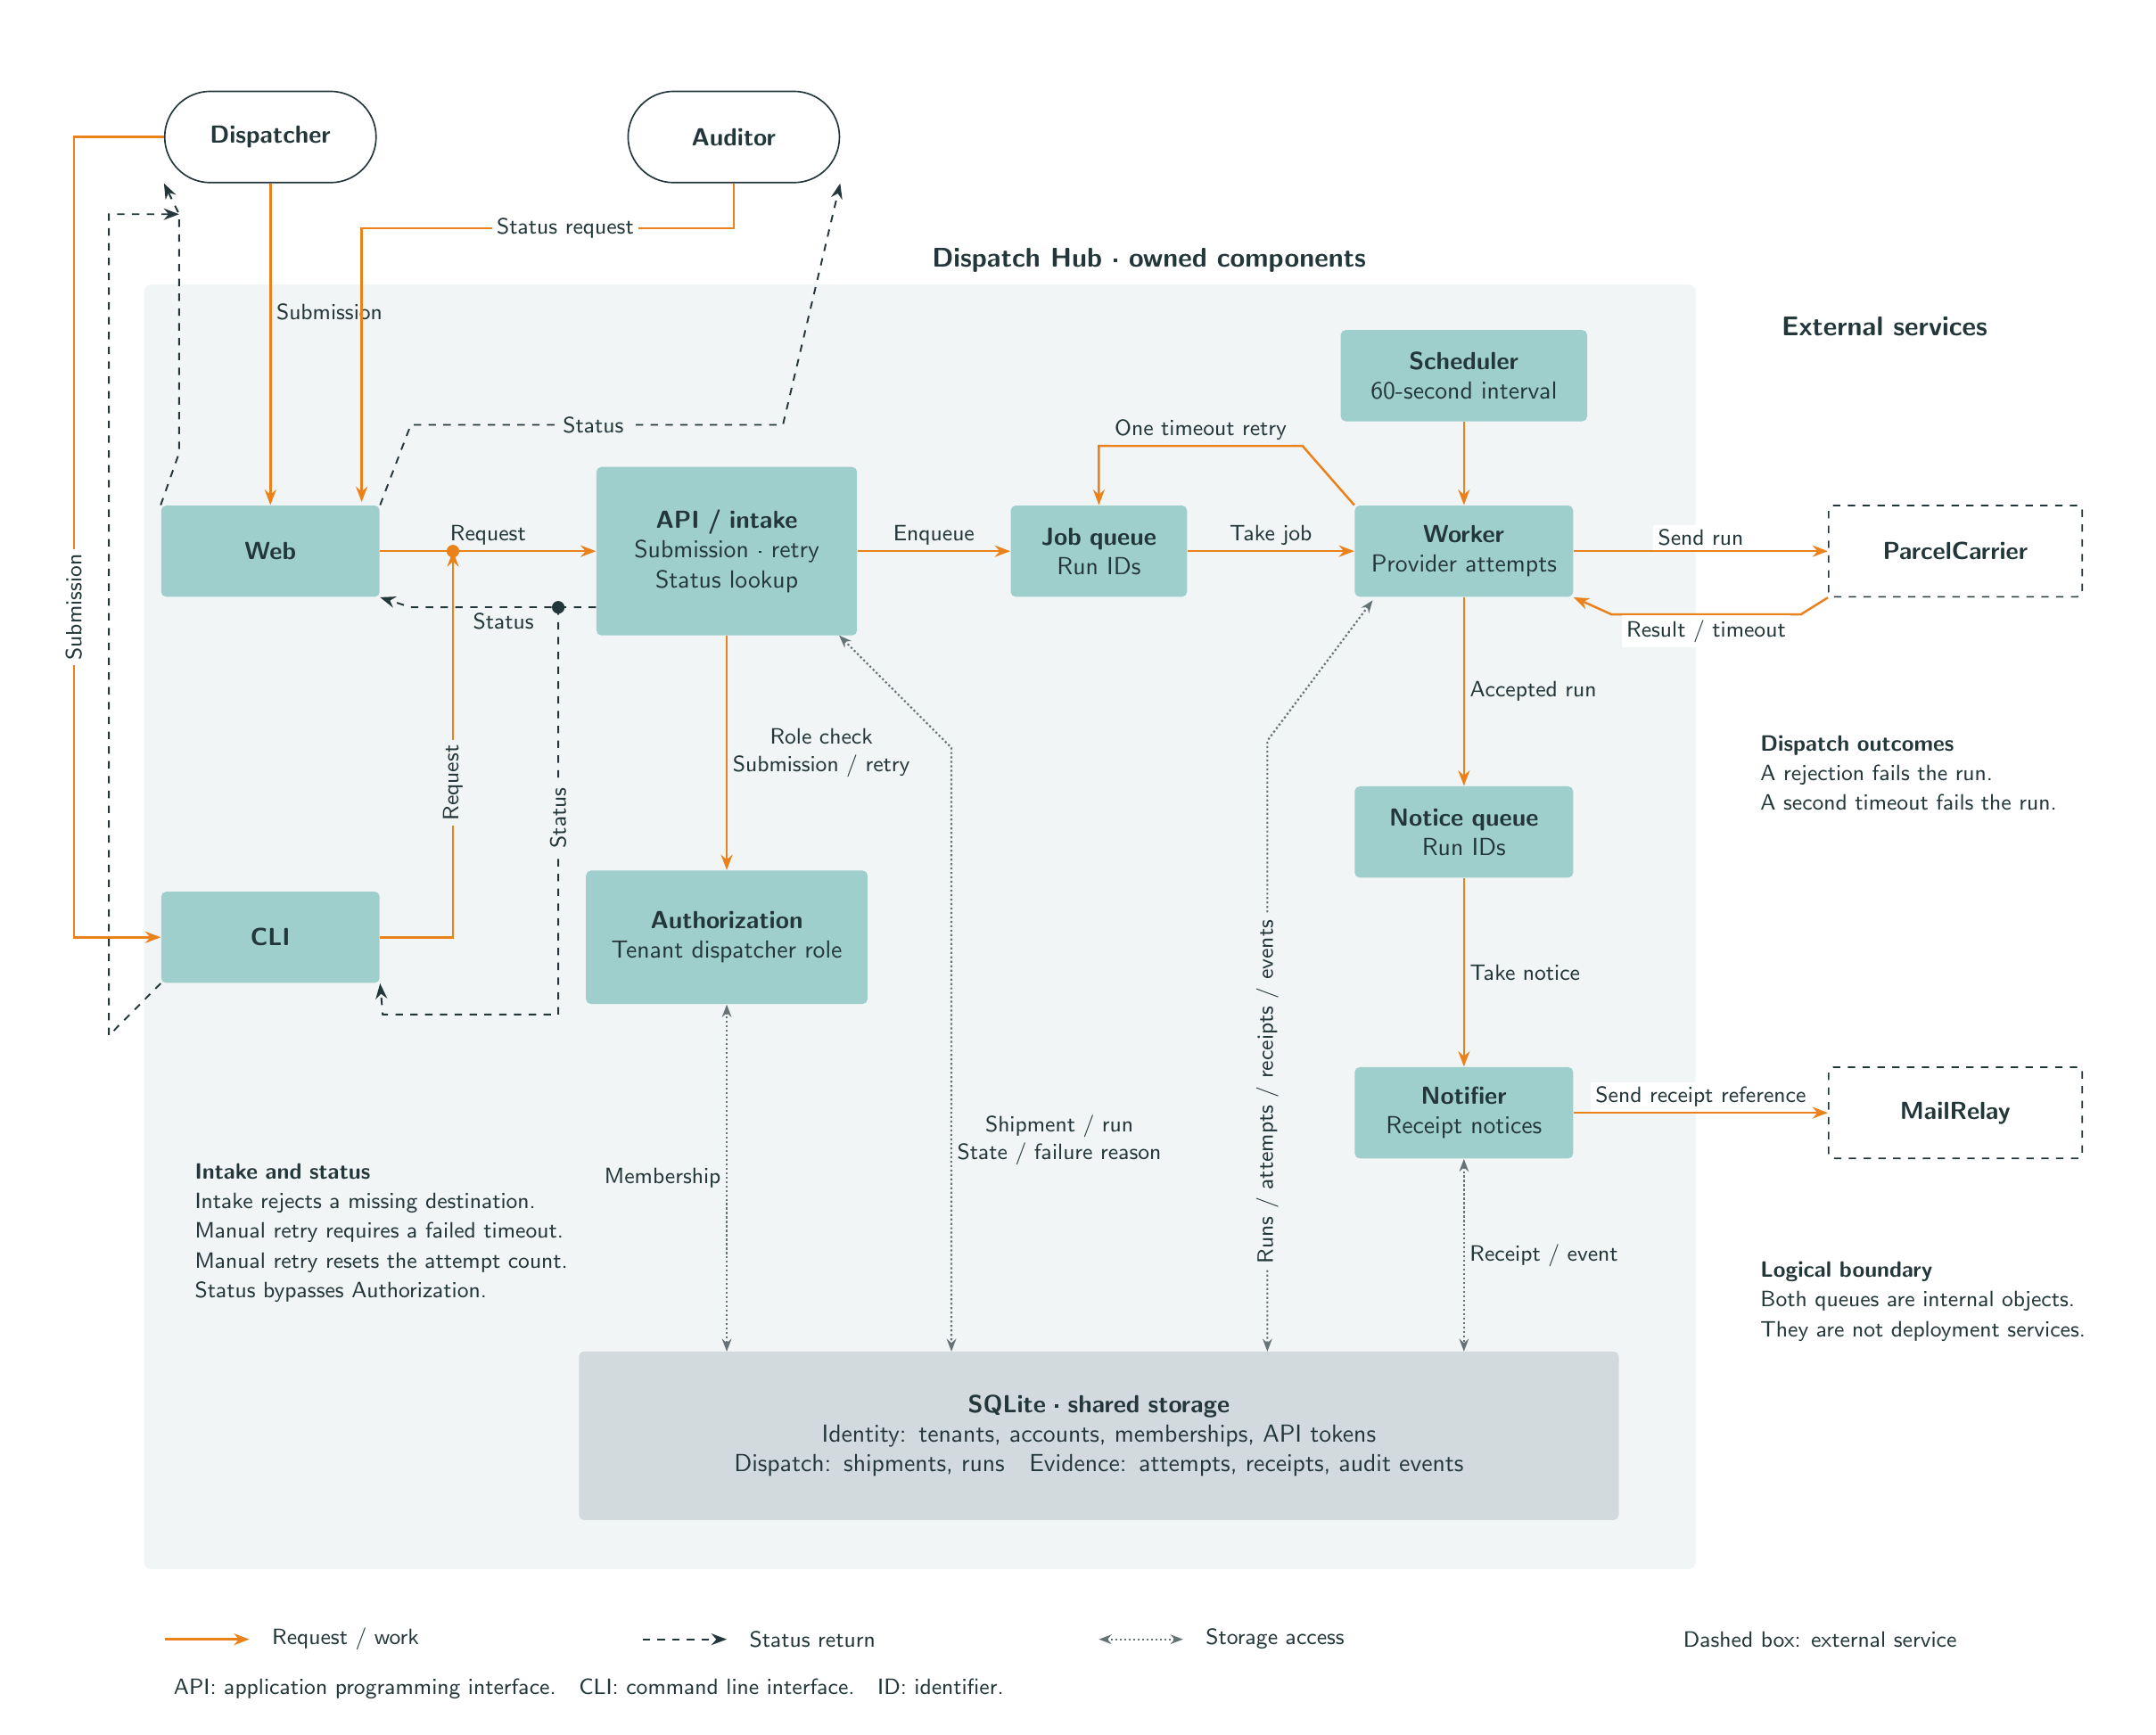
\begin{tikzpicture}[x=1mm,y=1mm,font=\sffamily\fontsize{10}{12}\selectfont,text=ink]
\path[use as bounding box] (0,0) rectangle (300,240);
\fill[zone,rounded corners=3pt] (17,20) rectangle (238,203);
\node[heading,anchor=south west] at (128,203.5) {Dispatch Hub · owned components};
\node[heading,anchor=west] at (249,197) {External services};
\node[actor] (dispatcher) at (35,224) {\textbf{Dispatcher}};
\node[actor] (auditor) at (101,224) {\textbf{Auditor}};
\node[component] (web) at (35,165) {\textbf{Web}};
\node[component] (cli) at (35,110) {\textbf{CLI}};
\node[component,text width=35mm,minimum height=24mm] (api) at (100,165) {\textbf{API / intake}\\Submission · retry\\Status lookup};
\node[component,text width=38mm,minimum height=19mm] (auth) at (100,110) {\textbf{Authorization}\\Tenant dispatcher role};
\node[component,text width=23mm] (jobs) at (153,165) {\textbf{Job queue}\\Run IDs};
\node[component] (worker) at (205,165) {\textbf{Worker}\\Provider attempts};
\node[component,text width=33mm] (scheduler) at (205,190) {\textbf{Scheduler}\\60-second interval};
\node[component] (notices) at (205,125) {\textbf{Notice queue}\\Run IDs};
\node[component] (notifier) at (205,85) {\textbf{Notifier}\\Receipt notices};
\node[external] (carrier) at (275,165) {\textbf{ParcelCarrier}};
\node[external] (mail) at (275,85) {\textbf{MailRelay}};
\node[box,fill=store,text width=146mm,minimum height=24mm] (db) at (153,39) {\textbf{SQLite · shared storage}\\Identity: tenants, accounts, memberships, API tokens\\Dispatch: shipments, runs\quad Evidence: attempts, receipts, audit events};
\draw[flow] (dispatcher.south) -- node[el,right,pos=.4]{Submission} (web.north);
\draw[flow] (dispatcher.west) -- (7,224) |- (cli.west);
\node[el,fill=white,rotate=90] at (7,157) {Submission};
\draw[flow] (auditor.south) -- (101,211) -| (48,211) -- (48,172);
\node[el,fill=white] at (77,211) {Status request};
\draw[status] (web.north east) -- (55,183) -- (108,183) -- (auditor.south east);
\node[el] at (81,183) {Status};
\draw[status] (web.north west) -- (22,179) -- (22,213) -- (dispatcher.south west);
\draw[status] (cli.south west) -- (12,96) -- (12,213) -- (22,213);
\draw[flow] (web.east) -- node[el,above]{Request} (api.west);
\draw[status] (api.west |- 0,157) -- node[el,below]{Status} (55,157) -- (web.south east);
\draw[flow] (cli.east) -- (61,110) -- (61,165);
\fill[accent] (61,165) circle (.9);
\node[el,rotate=90] at (61,132) {Request};
\draw[status] (76,157) -- (76,99) -- (51,99) -- (cli.south east);
\fill[ink] (76,157) circle (.9);
\node[el,rotate=90] at (76,127) {Status};
\draw[flow] (api.south) -- node[el,right]{Role check\\Submission / retry} (auth.north);
\draw[data] (auth.south) -- node[el,left]{Membership} (100,51);
\draw[data] (116,153) -- (132,137) -- node[el,right,pos=.65]{Shipment / run\\State / failure reason} (132,51);
\draw[flow] (api.east) -- node[el,above]{Enqueue} (jobs.west);
\draw[flow] (jobs.east) -- node[el,above]{Take job} (worker.west);
\draw[flow] (scheduler.south) -- (worker.north);
\draw[flow] (worker.north west) -- (182,180) -- node[el,above]{One timeout retry} (153,180) -- (jobs.north);
\draw[flow] (worker.south) -- node[el,right]{Accepted run} (notices.north);
\draw[flow] (notices.south) -- node[el,right]{Take notice} (notifier.north);
\draw[data] (192,158) -- (177,138) -- (177,51);
\node[el,rotate=90] at (177,88) {Runs / attempts / receipts / events};
\draw[data] (notifier.south) -- node[el,right]{Receipt / event} (205,51);
\draw[flow] (worker.east) -- node[el,fill=white,above]{Send run} (carrier.west);
\draw[flow] (carrier.south west) -- (253,156) -- node[el,fill=white,below]{Result / timeout} (226,156) -- (worker.south east);
\draw[flow] (notifier.east) -- node[el,fill=white,above]{Send receipt reference} (mail.west);
\node[note,anchor=north west,text width=66mm] at (23,79) {\textbf{Intake and status}\\Intake rejects a missing destination.\\Manual retry requires a failed timeout.\\Manual retry resets the attempt count.\\Status bypasses Authorization.};
\node[note,anchor=north west,text width=53mm] at (246,140) {\textbf{Dispatch outcomes}\\A rejection fails the run.\\A second timeout fails the run.};
\node[note,anchor=north west,text width=53mm] at (246,65) {\textbf{Logical boundary}\\Both queues are internal objects.\\They are not deployment services.};
\draw[flow] (20,10) -- (32,10);\node[note,anchor=west] at (34,10) {Request / work};
\draw[status] (88,10) -- (100,10);\node[note,anchor=west] at (102,10) {Status return};
\draw[data] (153,10) -- (165,10);\node[note,anchor=west] at (167,10) {Storage access};
\node[note,anchor=west] at (235,10) {Dashed box: external service};
\node[note,anchor=west] at (20,3) {API: application programming interface.\quad CLI: command line interface.\quad ID: identifier.};
\end{tikzpicture}
\end{document}
